\documentclass[italian,12pt,a4paper,oneside,final]{report}
%\documentclass[italian,a4paper,titlepage]{article}
%\usepackage{amsmath}
%\usepackage{caption}
%\usepackage{subcaption}
\usepackage{graphicx}
\usepackage{biblatex} %Imports biblatex package
\usepackage[utf8]{inputenc}
\usepackage[italian]{babel}
\usepackage{csquotes}
%\usepackage[T1]{fontenc}
%\usepackage{longtable}
%\usepackage{booktabs}
%\usepackage{textcomp}
%\usepackage[draft=false]{hyperref}
%\usepackage{hyperref}
%\usepackage[table]{xcolor}
\addbibresource{iot.bib} %Import the bibliography file
\graphicspath{ {images/} }
\renewcommand{\thesection}{\arabic{section}} % remove the \chapter counter from being printed with every \section
%\hypersetup{
%	colorlinks=true,
%	linkcolor=,
%	pdftitle={Marco Giunta - Progetto IoT},
%	pdfauthor={Marco Giunta},
%}

\title{\huge Power Meter Wi-Fi con Arduino\\[0.5em]
\large Relazione Progetto IoT}
\date{Ottobre 2022}
\author{
Marco Giunta\thanks{Marco Giunta 147852 giunta.marco@spes.uniud.it}}

\begin{document}
% Generate title page
\maketitle

% Generate TOCs
\pagenumbering{arabic}
\tableofcontents

\newpage

\section{Introduzione}
Una delle sfide chiave del XXI secolo è l’adattamento ai cambiamenti climatici.
Per riuscire a limitare il riscaldamento globale, è necessario impiegare l’energia in modo efficiente, riducendo il consumo all'interno delle proprie abitazioni o negli edifici pubblici.
Per poter decidere quali misure adottare, è indispensabile conoscere il consumo reale delle apparecchiature che usiamo ogni giorno.

Con questo progetto si vuole realizzare un prototipo a basso costo di un misuratore di consumo elettrico collegato ad una rete locale tramite Wi-Fi.
Il progetto ha come obiettivo l’acquisizione e il monitoraggio dei valori di tensione, corrente e potenza presenti ai capi di un qualunque apparecchio collegato alla rete elettrica domestica (220V).
Il codice presente all'interno del dispositivo è stato progettato per permettere il collegamento contemporaneo di circa 65.000 unità, per essere in grado di monitorare, ad esempio, tutte le apparecchiature presenti all'interno di un istituto di ricerca.

Per garantire il monitoraggio di un numero così elevato di dispositivi, è stato necessario ricorrere all'utilizzo del protocollo MQTT\footfullcite{mqtt}, per ottimizzare la gestione della banda di rete e garantire l'autenticazione dei singoli dispositivi.
Per raccogliere i dati è stato utilizzato il sistema di gestione di database InfluxDB\footfullcite{influxdb} mentre, per la parte di visualizzazione tramite dashboard, è stato utilizzato il software Grafana\footfullcite{grafana}.

A solo scopo dimostrativo, il broker Mosquitto\footfullcite{mosquitto}, il collettore Telegraf\footfullcite{telegraf}, InfluxDB e Grafana sono stati configurati, utilizzando la tecnologia dei container, in una scheda single-board ARM Orange Pi PC 2 con sistema operativo Fedora IoT.

\newpage

\section{Componenti}
Per la realizzazione del prototipo sono stati utilizzati questi componenti:

\begin{itemize}
\item Arduino MKR1000
\item Display LCD 16×2
\item Modulo LCM1602 IIC per display LCD
\item Sensore di Corrente AC-CC da 5A con ACS712
\item Sensore di tensione con ZMPT101B
\item Divisori di tensione (da 5V a 3.3V)
\end{itemize}


\subsection{Schema elettrico}
\begin{figure}[h]
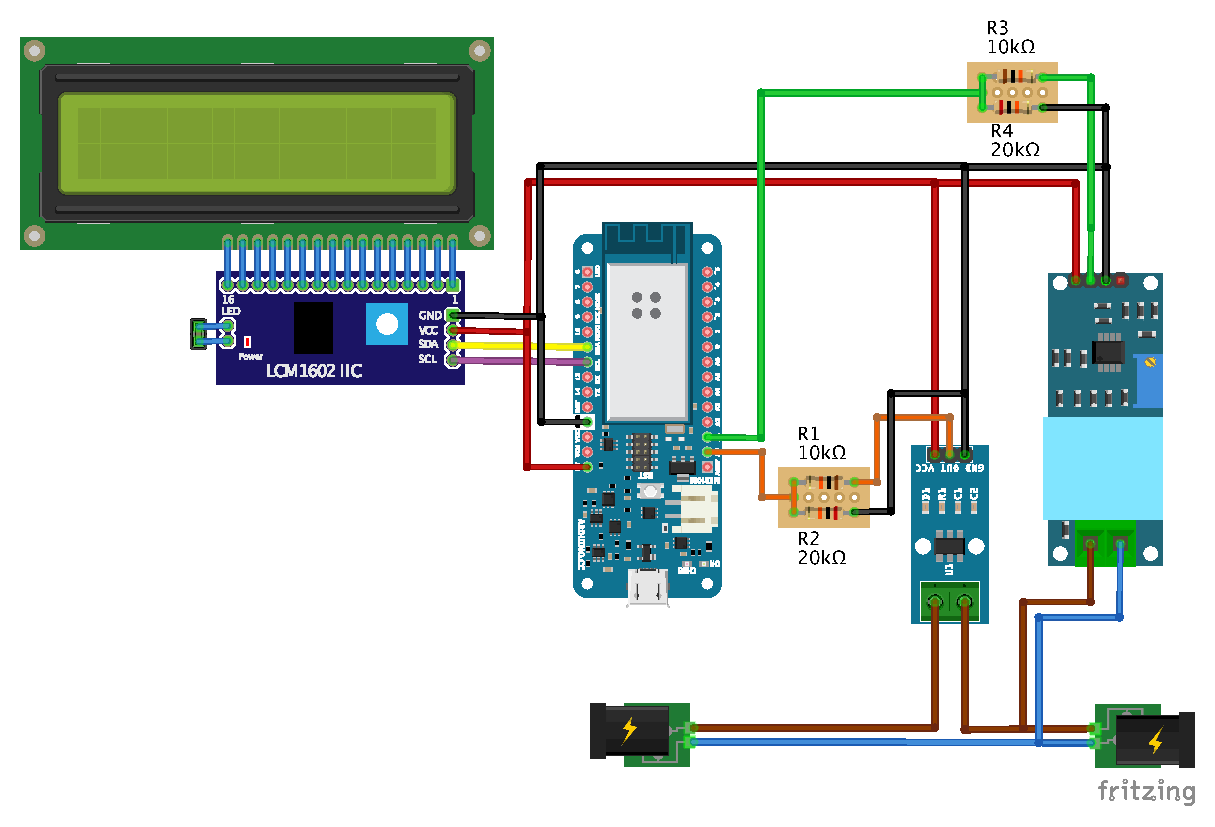
\includegraphics[width=\textwidth]{power_meter_bb.pdf}
\centering
\end{figure}

Lo scopo di questa settima esperienza di laboratorio è determinare i valori delle costanti di taratura della funzione di trasferimento di un sensore di temperatura, usato come trasduttore tra le grandezze temperatura e resistenza.
Misureremo la temperatura di un bagno termico attraverso un termometro ad alcool e una serie di termistori NTC.
Inoltre determineremo il tempo di risposta di uno dei termistori NTC utilizzati durante l'esperimento.

\subsection{Trasduzione di grandezze fisiche}
In tutti i casi in cui si vuole misurare una grandezza fisica, ma non è possibile confrontarla con uno o più campioni o definirla mediante una misura indiretta, si ricorre alla \emph{correlazione} della grandezza fisica con un’altra, più semplice da misurare.
I dispositivi che permettono questo tipo di correlazione (\emph{trasduzione}) vengono chiamati \textbf{trasduttori}.
\end{document}